\clearpage
\makeatletter
\efloat@restorefloats
\makeatother


\begin{appendix}
\section{}
Some general data properties, which are needed to determine the most
appropriate analytical approach, were examined. The absence of
multivariate normality in all items (Mardia's Test: sig. \textless{}
.01), and missing data (11.3\% of the cases, with a completely random
distribu- tion of the missing data; Little's test sig. p \textgreater{}
.05) were observed. Given the ordinal nature of the data, the weighted
least square with adjusted mean and variance (WLSMV) (Beauducel \&
Herzberg, 2006; Rhemtulla et al., 2012) approach was used as an
estimation method of the factor models.

In all studied models, goodness of fit was determined by using the
comparative fit index (CFI), the Tucker- Lewis index (TLI) and the root
mean square of approxi- mation (RMSEA). For the CFI and TLI, values
above .90 and .95, respectively, indicate an acceptable and adequate fit
(Chen, 2007, Hu \& Bentler, 1999). In the case of the RMSEA, values
below .08 and .05, respectively, indicate an acceptable and appropriate
fit (Cheung \& Rensvold, 2002). To determine the significance of the fit
differences between the nested or equivalent models, Chen (Chen, 2007)
and Cheung and Resvold's (Cheung \& Rensvold, 2002) recommendations were
followed. According to these scholars, increases in the CFI and TLI less
than .01 and decreases in the RMSEA less than .015 suggest that there
are no substantial differences in fit among the com- pared models. All
analyses were performed by using MPlus v 7.3 (Muthén \& Muthén, 2014).

The following data analytic strategy was adopted. First, six measurement
models were estimated via ICM-CFA (independent clusters model of
confirmatory factor analysis). Second, and based on the results from the
previous step, an ESEM model with a similar configuration to the
four-correlated-factor structure proposed by the DSM--5 was estimated.
Third, an ESEM bifactor model was estimated to explore the existence of
a common source of variance to all PTSD symptoms. To estimate the
model-based reliability for each factor the omega index was calculated
in the case of the first order models (McDonald, 1999). The omega
hierarchical index (Zinbarg et al., 2006) and the omega sub-scale were
estimated in the case of the bifactor model (Reise, 2012). These indexes
quantify the degree to which the factor scores accurately reflect the
position of the subject in the latent variable (values above .70 are
required to ensure the psychometric interpretability of the factor). To
estimate the internal consistency of each factor, Cronbach's alpha was
used.

\begin{figure}
\centering
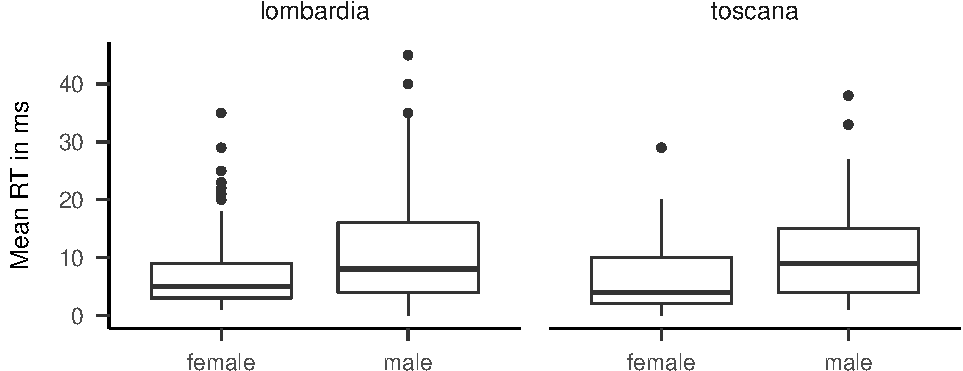
\includegraphics{self_compassion_files/figure-latex/unnamed-chunk-23-1.pdf}
\caption{(\#fig:unnamed-chunk-23)Boxplots of mean response times for all
fast tasks, split by age groups. See Table 1 for an explanation of the
task names.}
\end{figure}
\end{appendix}
